\documentclass[a4paper,12pt]{article}

\usepackage{cmap}                   
\usepackage{mathtext}     
\usepackage{amssymb,amsmath}
\usepackage{tipx}
\usepackage{algorithm2e}
\usepackage{listings}
%изображения
\usepackage{graphicx}%Вставка картинок правильная
\usepackage{float}%"Плавающие" картинки
\usepackage{wrapfig}%Обтекание фигур (таблиц, картинок и прочего)

\usepackage[T1,T2A]{fontenc}        
\usepackage[utf8]{inputenc}         
\usepackage[english, russian]{babel} 
\usepackage[top=0.35in, bottom=0.5in, left=0.3in,right=0.3in]{geometry}

\newtheorem{theorem}{Теорема}
\newtheorem{proposal}{Предположение}
\newtheorem{notice}{Замечание}
\newtheorem{statement}{Положение}
\newtheorem{corollary}{Следствие}
\newtheorem{lemma}{Лемма}
\newtheorem{observation}{Наблюдение}
\newtheorem{problem}{Задача}
\newtheorem{claim}{Решение}

\title{Графы, II семестр, краткое содержание}
\author{Проскуряков Иван КМБО-02-19}
\begin{document}

    \maketitle
    \section{Стандартные обозначения:}
        \begin{itemize}
          \item $Г$ - граф
          \item $E$ - множество рёбер графа
          \item $V$ - множество вершин графа
          \item $Р$ - мощность множества рёбер
          \item $В$ - мощность множества вершин
          \item $F$ - множество граней графа
          \item $S:\overrightarrow{E} \rightarrow V$ - функция, возвращающая начало ребра
          \item $t:\overrightarrow{E} \rightarrow V$ - функция, возвращающая конец ребра
        \end{itemize}

    \section{Определения:}
        \begin{enumerate}
            \item \textbf{Граф}:
                \begin{itemize}
                    \item Определим граф без кратных рёбер и петель: 
                    $$
                    E \subset V \times V 
                    $$
                    (Иными словами, множество рёбер определяется как подмножество прямого произведения множества вершин графа с собой)
                    \item Определим граф с кратными рёбрами и петлями(обычно в литературе их называют "мультиграфами" и "псевдографами" соответственно):
                    
                    $\qquad$Пусть $E$ - некоторый набор отрезков, $\delta E$ - множество концов отрезков, $\mathfrak{R}$ - отношение эквивалентности на $\delta E$, тогда вершины являются некоторыми классами эквивалентности.
                \end{itemize} 
                
            \item \textbf{Матрица смежности} - матрица размерности $Р\times Р$, где на позиции с индексом $i, j$ (номер строки, номер столбца соответственно) стоит 1, если $i-ая$ и $j-ая$ вершины пересекаются (т.е. существует ребро, связывающее их), иначе стоит 0.
            \item \textbf{Матрица инциденции} - матрица размерности $В\times Р$(пусть это матрица $H^{В\times Р}$), где строки соответствуют вершинам графа, столбцы - рёбрам графа. Соответственно, в ячейке $h_{i j}$ будет указано отношение инциденции для i-ой вершины и j-ого ребра графа. 

            $\qquad$Напомним, что ребро и вершина находятся в отношении \textbf{инциденции}, если \textit{вершина лежит на заданном ребре}.
            
            $\qquad$Если граф ненаправленный, имеем:
                 \begin{equation*}
                    h_{i j} = 
                   \begin{cases}
                       1,  \text{ если вершина } v_i \text{ инцидентна ребру } e_j\\
                       0, \text{ в противном случае}
                   \end{cases}
                \end{equation*} 
            \begin{figure}[ht]

                    \centering
                    
                    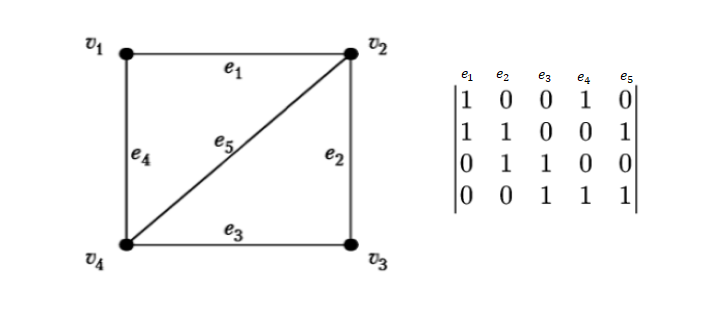
\includegraphics[scale=0.8]{ex1.png}
                    
                    \caption{Пример ненаправленного графа с матрицей инциденции}
                    
                    \label{fig:gn}
                
            \end{figure}
            $\qquad$Если направленный:
                 \begin{equation*}
                    h_{i j} = 
                   \begin{cases}
                       1,  \text{ если вершина } v_i \text{ инцидентна ребру } e_j 
                       \text{ и является его концом}\\
                       0, \text{ вершина }v_i \text{ не инцидентна ребру } e_j\\
                       -1, \text{ если вершина } v_i \text{ инцидентна ребру } e_j 
                       \text{ и является его началом}
                   \end{cases}
                \end{equation*} 
            \begin{figure}[ht]

                    \centering
                    
                    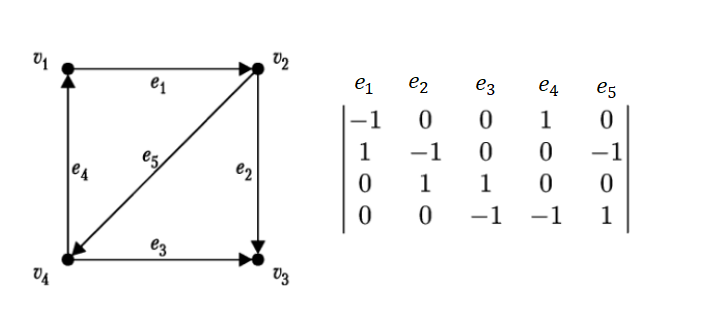
\includegraphics[scale=0.7]{ex2.png}
                    
                    \caption{Пример направленного графа с матрицей инциденции}
                    
                    \label{fig:gd}
                
            \end{figure}
            
            \item \textbf{Путь} $\overrightarrow l$ в графе - набор рёбер $\overrightarrow l = (\overrightarrow e_1, \overrightarrow e_2, \cdots, \overrightarrow e_n)$ таких, что $t(\overrightarrow e_i) = S(\overrightarrow e_{i+1})$  $\forall i \in$ $\{1, 2, \cdots, n - 1\}$.
            \item \textbf{Простой путь} - путь, в котором каждое из рёбер графа пройдено не более одного раза.
            \item \textbf{Ориентированное ребро} - ребро, имеющее направление.
            \item \textbf{Число рёберной связности} $\lambda$ - минимальное число рёбер, при удалении которых граф перестанет быть связным. 
            \item \textbf{Число вершинной связности} $\textipa{\textsl{@e}}$
            - наименьшее число вершин, при удалении которых граф потеряет связность или станет одновершинным.
            \item \textbf{Валентность (степень) вершины }$\nu(a)$ - определяет, сколько концов рёбер входит в вершину $a$. 
            \item \textbf{Паспорт графа} - матрица $1\times В$, где на i-ой позиции задаётся валентность i-ой вершины.
            \item \textbf{Изоморфизм графов} - Пусть $Г$ и $Г^\prime$ - два графа, а отображение $\phi : V(Г) \rightarrow V(Г^\prime)$ таково, что $x y \in E(Г) \Leftrightarrow \phi (x) \phi(y) \in E(Г^\prime)$. Тогда $\phi$ - изоморфизм графов $Г$ и $Г^\prime$, а сами графы изоморфны.
            
            $\qquad$ \textit{Пояснение:} $x,y$ - в данном случае некоторые вершины графа $Г$, соответственно $x y$ - некоторое ребро, связывающее эти две вершины. Отображение $\phi$ переводит вершины $x, y$ графа $Г$ в некоторые вершины графа $Г^\prime$, для простоты назовём их $x^\prime, y^\prime$. Но тогда $x^\prime = \phi (x), y^\prime = \phi(y)$; теперь очевидно, что $\phi (x) \phi(y)$  - это некоторое ребро, связывающее вершины $x^\prime$ и $y^\prime$, и если это ребро является ребром графа $(Г^\prime)$, то отображение $\phi$ будет изоморфизмом.
            
            \item \textbf{Дерево} - связный граф, не имеющий циклов.
            
            $\qquad$ \textit{Пояснение 1:} \textbf{связным} называется граф такой, что из любой вершины графа существует путь в любую другую.
            
            $\qquad$ \textit{Пояснение 2:} \textbf{циклом} называется путь $\Vec{l} = (\Vec{e_1}, \Vec{e_2}, \cdots, \Vec{e_n}): S(\Vec{e_1}) = t(\Vec{e_n})$ (то есть вершина отправления является вершиной окончания пути).
            
            $\qquad$ \textit{Пояснение 3:} Это не строгое определение дерева, $\exists$ 4 строгих эквивалентных определения. Все они будут приведены в следующем разделе.
            \item \textbf{Мост, компонента связности:}
                
            $\qquad$ \textit{Пояснение:} понятие моста вводилось в семестре в довольно наивной формулировке, поэтому здесь будет приведена более строгая, хотя и с использованием терминов, не вводившихся лектором.
                \begin{itemize}
                    \item \textbf{Компонентой связности} называется связный подграф. Говоря строже, это такой набор вершин графа, между любой парой которых можно проложить путь.
                    \item \textbf{Мостом} называется ребро, удаление которого увеличивает количество компонент связности.
                \end{itemize}
            
            \item \textbf{Остовное дерево} $\Delta$  - дерево, содержащее все вершины некоторого графа.
            \begin{figure}[ht]

                    \centering
                    
                    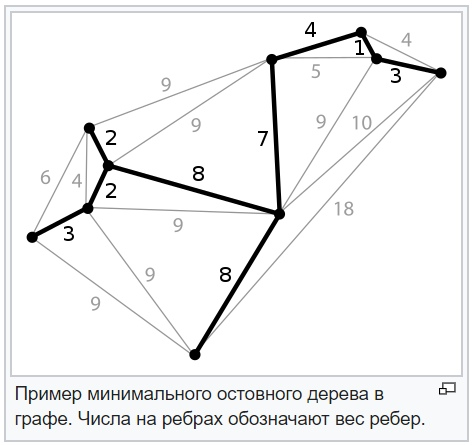
\includegraphics[scale=0.7]{ex3.jpg}
                    
                    \caption{}
                    
                    \label{fig:ct}
                
            \end{figure}
            
            \item \textbf{Полный граф} - граф, в котором любые две вершины являются смежными.
            \item \textbf{Двудольный граф} - граф, множество вершин которого может быть разбито на два непересекающихся множества ($V_1, V_2: V_1 \cup V_2 = V, V_1 \cap V_2 = \emptyset$), причём всякое ребро из $E$ инцидентно вершине из $V_1$ и вершине из $V_2$.
            \item \textbf{Полный двудольный граф} - двудольный граф, содержащий все рёбра, соединяющие множества $V_1$ и $V_2$.
            
            $\qquad$ Пусть $В_1 = m, В_2 = n$, тогда полный двудольный граф обозначается $K_{m, n}$.
            \begin{figure}[ht]

                    \centering
                    
                    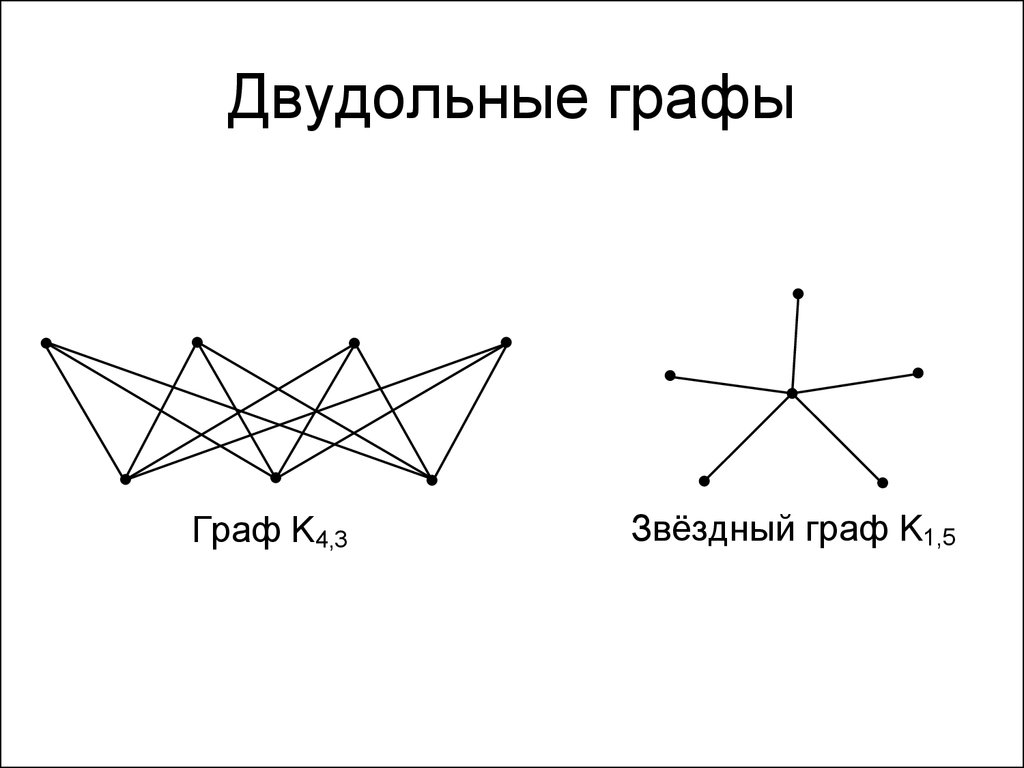
\includegraphics[scale=0.5]{seal.jpg}
                    
                    \caption{Примеры двудольных графов (полных)}
                    
                    \label{fig:mpr}
                
            \end{figure}
            \item \textbf{Планарный граф} - граф, который можно изобразить на плоскости так, чтобы его рёбра не пересекались во внутренних точках.
            
            $\qquad$ Иными словами, это такой граф, который можно реализовать как симплициальный комплекс с нулевыми вторыми гомологиями из симплексов размерности два.
            \begin{figure}[ht]

                    \centering
                    
                    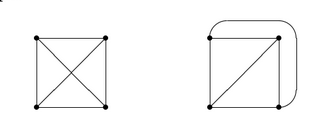
\includegraphics[scale=0.7]{ex4.png}
                    
                    \caption{Планарный краф $K_4$ и его укладка на плоскость}
                    
                    \label{fig:K4}
                
            \end{figure}
            
            \item \textbf{Грани графа} - части, на которые \textit{плоский граф} (т.е. граф в изображении на плоскость, неважно, пересекаются его рёбра во внутренних точках или нет) делит плоскость.
            
            \begin{figure}[ht]

                    \centering
                    
                    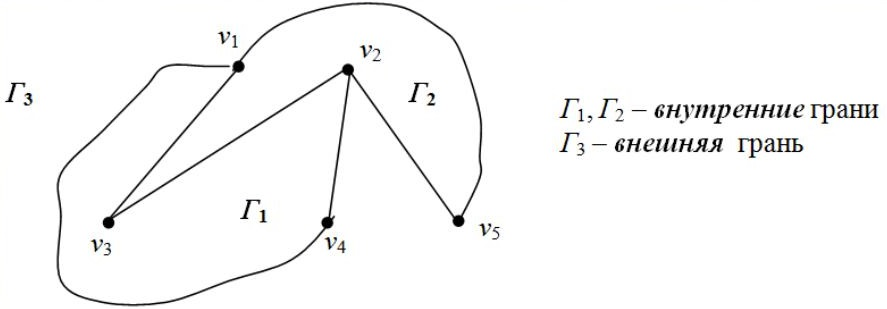
\includegraphics[scale=0.7]{ex5.jpg}
                    
                    \caption{Иллюстрация к понятию граней графа}
                    
                    \label{fig:GB}
                
            \end{figure}
            \item \textbf{Правильно вложенный в плоскость граф} - граф, грани которого на плоскости есть многоугольники.
            \item \textbf{Цикломатическое число графа} $g(Г) = Р - В + 1$.
            
            $\qquad$ \textit{Замечание:} Единица в данном равенстве есть количество компонент связности в данном графе. В данном курсе это понятие не рассматривается, но осознавать его стоит. Выше дано его определение.
            \item \textbf{Гомеоморфность графа} - граф называется гомеоморфным, если он получен путём стягивания рёбер или долбавлением вершин на существующие рёбра.
            \begin{figure}[ht]

                    \centering
                    
                    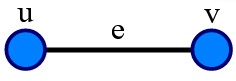
\includegraphics[scale=0.7]{ex61.png}
                    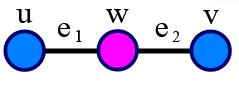
\includegraphics[scale=0.7]{ex62.png}
                    \caption{Пример гомеоморфных графов}
                    
                    \label{fig:GG}
                
            \end{figure}
        \end{enumerate}
        %\newpage
    \section{Теоремы и алгоритмы:}
        \begin{enumerate}
            \item \textbf{Алгоритмы нахождения кратчайшего пути в графе} - Алгоритм Дейкстры(для взвешенного графа) и алгоритм поиска в ширину(для не взвешенного графа):
        
            \textit{Пояснение 1:} \textit{взвешенным} графом называется граф, рёбра которого имеют определённую цену (цена - она же вес ребра).
            \begin{enumerate}
                \item \textbf{Алгоритм Дейкстры:}
                    \begin{itemize}
                        \item Словесное описание:
                        \begin{enumerate}
                            \item Найти узел с наименьшей стоимостью (то есть узел, за который можно добраться за минимальную цену).
                            
                            $\qquad$ \textit{Замечание 1:} перед тем, как обходить граф, в котором ещё не известна стоимость ни одной вершины, необходимо узел отправления пометить ценой ноль, остальные получат стоимость $\infty$. 
                            \item Обновить стоимость соседей этого узла.
                            
                            $\qquad$ \textit{Пример:} пусть $V_1$ - вершина со стоимостью 4. $V_3$ - вершина со стоимостью $15$ (возможно, эта цена была получена, когда в эту вершину мы попали по другому пути, а, возможно, такая цена была установлена изначально). Эти две вершины связаны друг с другом ребром стоимостью 6. Совершенно логично, что $4 + 6 < 15, \Rightarrow$ новая цена $V_3$ будет $4 + 6 = 10$.
                            \item Перейти снова к пункту i и повторять до тех пор, пока все узлы графа не будут оценены.
                            \item Вычислить итоговый путь.
                        \end{enumerate}
                        \item Псевдокод: 
                    \end{itemize}
                    \lstset{language=Python, keepspaces = true, extendedchars=\false}
                    \lstinputlisting[language=Python]{main.py}
                \item \textbf{Алгоритм поиска в ширину} (словесное описание):
                    \begin{enumerate}
                        \item Расставляем метки вершинам графа: $V_1 - \text{метка 1}, V_2$ - вершина, смежная с предыдущей, получает метку 2, $\cdots$
                        \item На k-ом шаге метку k+1 получат вершины, которые либо ещё не имеют метки, либо являются смежными с вершиной k.
                        \item Если на некотором шаге не нашлось вершин из предыдущего пункта, и последняя вершина, до которой удалось дойти, не является пунктом назначиения, то граф несвязный. Иначе последняя вершина - $t(e_n)$.
                    \end{enumerate}
            \end{enumerate}
            \item \textbf{Жадный алгоритм:}
            
            \textit{Пояснение 2:} используется для нахождения минимального и максимального остовного дерева.
            
            \textit{Пояснение 3:} \textbf{минимальным остовным деревом} будем называть дерево, сумма рёбер которого минимальна среди всех остовных деревьев данного графа.
            \begin{enumerate}
                \item Найти самое дешёвое (самое дорогое) ребро в графе. Если таких несколько - берём любое.
                \item Ищем самоё дешёвое (самое дорогое) реброе среди рёбер, смежным с ребром из предыдущего пункта. Берём его.
                \item Проверяем, не вошли ли мы в цикл. Если вошли - выбираем другое смежное ребро.
                \item Повторяем алгоритм до тех пор, пока не обойдём все вершины.
            \end{enumerate}
            \item 
                \begin{theorem}[Лемма о рукопожатиях]
                    Данный набор натуральных чисел является паспортом \textbf{какого-нибудь графа} $\Leftrightarrow$ сумма всех валентностей - всех чисел данного набора -  является чётной.
                \end{theorem}
                \begin{corollary}
                    Количество вершин с нечётным количеством валентностей всегда чётно.
                \end{corollary}
            \item 
                \begin{theorem}[Необходимое и достаточное условие для связности графа]
                    Граф с данным паспортом является связным 
                    $$
                    \Leftrightarrow \sum_{i=1}^n \left(\nu_i - 2\right) + 2 \geq 0
                    $$
                    Где $\nu_i$ - валентность i-ой вершины. 
                \end{theorem}
                \begin{notice}
                    $g(Г) = 0 \Leftrightarrow $ граф является деревом.
                \end{notice}
            
            \item \textbf{Цикломатическое число} вычисляется по следующим эквивалентным формулам: 
            $$
                g(Г) = \sum_{i=1}^n \left(\nu_i - 2\right) + 2 = Р - В + 1 \geq 0
            $$
            \item \begin{theorem}[Об эквивалентности определений дерева]
            Следущие 4 определения дерева эквивалентны:
                     \begin{enumerate}
                         \item $В = Р + 1$
                         \item При удалении $\forall$ ребра граф теряет связность ($\Leftrightarrow \forall$ ребро является мостом)
                         \item $\forall a, b \in V$ $\exists ! $ $\Vec{l}$, причём $\Vec{l}$ - простой путь.
                         \item В графе нет простых замкнутых путей.
                         \textit{Пояснение:} \textit{замкнутым} называется путь, точка отправления которого является и точкой прибытия.
                     \end{enumerate}
                \end{theorem}
            \item 
                \begin{theorem}[Связь чисел вершнинной связности $\textipa{\textsl{@e}}$ и рёберной связности $\lambda$]
                    $$
                    \lambda \geq \textipa{\textsl{@e}}
                    $$
                \end{theorem}
            \item 
                \begin{theorem}[Критерий эйлеровости графа]
                    Граф является эйлеровым, если либо все степени вершин чётны, либо количество вершин с нечётной степенью $\leq 2$. 
                    \begin{notice}
                        Эйлеров граф - граф, который можно обойти, пройдя каждое ребро не более одного раза.
                    \end{notice}
                \end{theorem}
            \item 
                \begin{theorem}[Критерий двудольности графа]
                    Все циклы в графе имеют чётную длину. 
                \end{theorem}
            \item 
                \begin{theorem}[Теорема Эйлера о планарных графах]
                    Для $\forall$ планарного графа выполняется:
                    $$
                    В - Р + Г = 2
                    $$
                    Где $Г$ - количество граней графа.
                \end{theorem}
            \item 
                \begin{theorem}[О непланарности $V_5$, $V_{3, 3}$]
                    Графы $V_5$, $V_{3, 3}$ непланарны.
                    \begin{notice}
                    $V_5$ - полный граф на 5 вершинах. $V_{3, 3}$ - полный двудольный граф: ситуация 'Три соседа - три колодца'.
                    \end{notice}
                \end{theorem}
                \begin{figure}[ht]
                    \centering
                    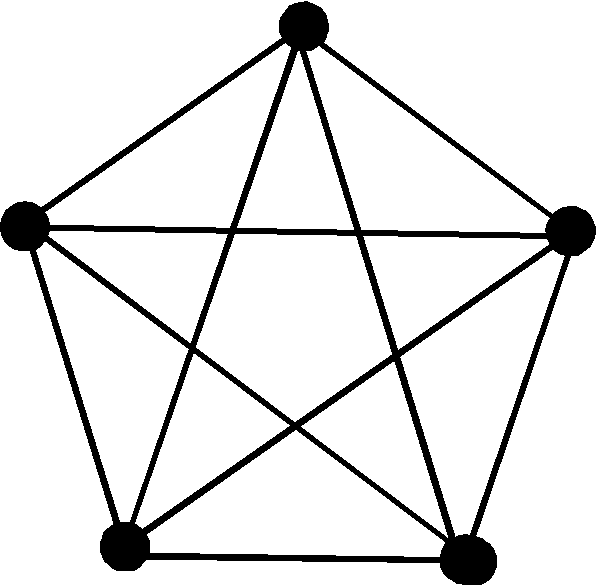
\includegraphics[scale=0.3]{ex71.png}
                    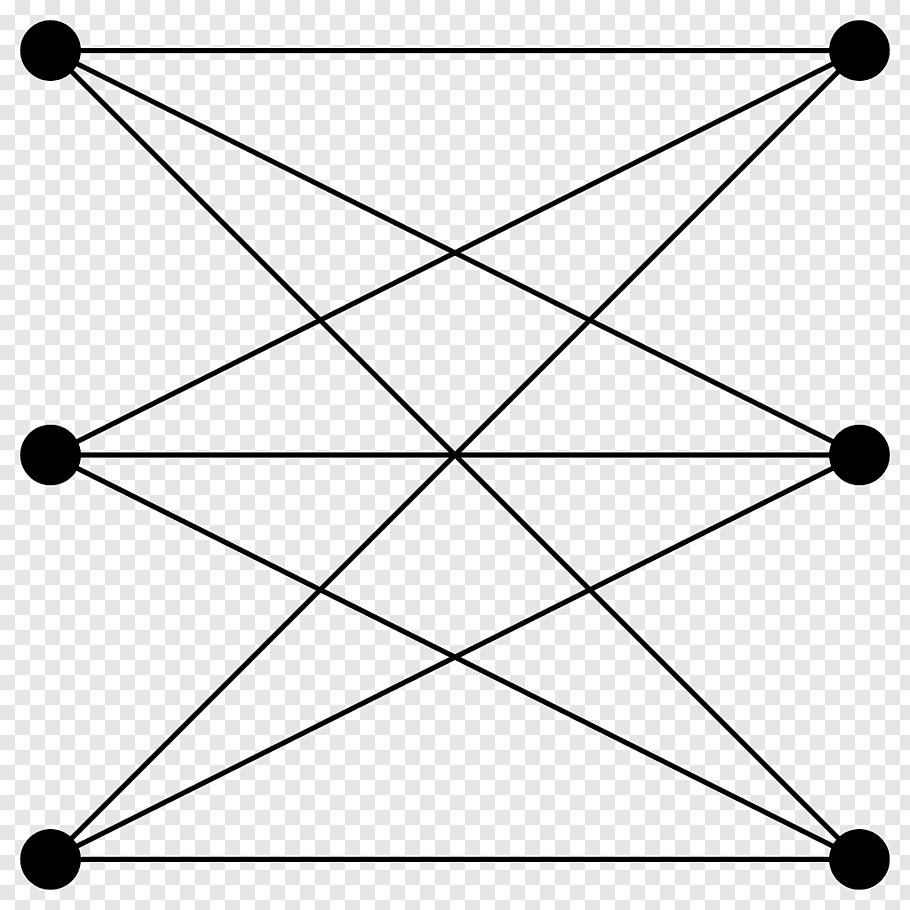
\includegraphics[scale=0.2]{ex72.png}
                    \caption{$V_5, V_{3, 3}$}
                    \label{fig:V5V33}
                \end{figure}
            
            \item
                \begin{theorem}[Теорема Понтрягина-Куратовского]
                    Граф не планарен $\Leftrightarrow$ в нем $\exists$ подграф, гомеоморфнаый либо $V_5$, либо $V_{3,3}$.
                \end{theorem}
        \end{enumerate}

\newpage
Список используемой литератруры:
\begin{itemize}
    \item Ф. А. Новиков - 'Дискретная математика для программистов'
    \item Д.В. Карпов - 'Теория графов'
    \item Адитья Бхаргава - 'Грокаем алгоритмы'
\end{itemize}
\end{document}
